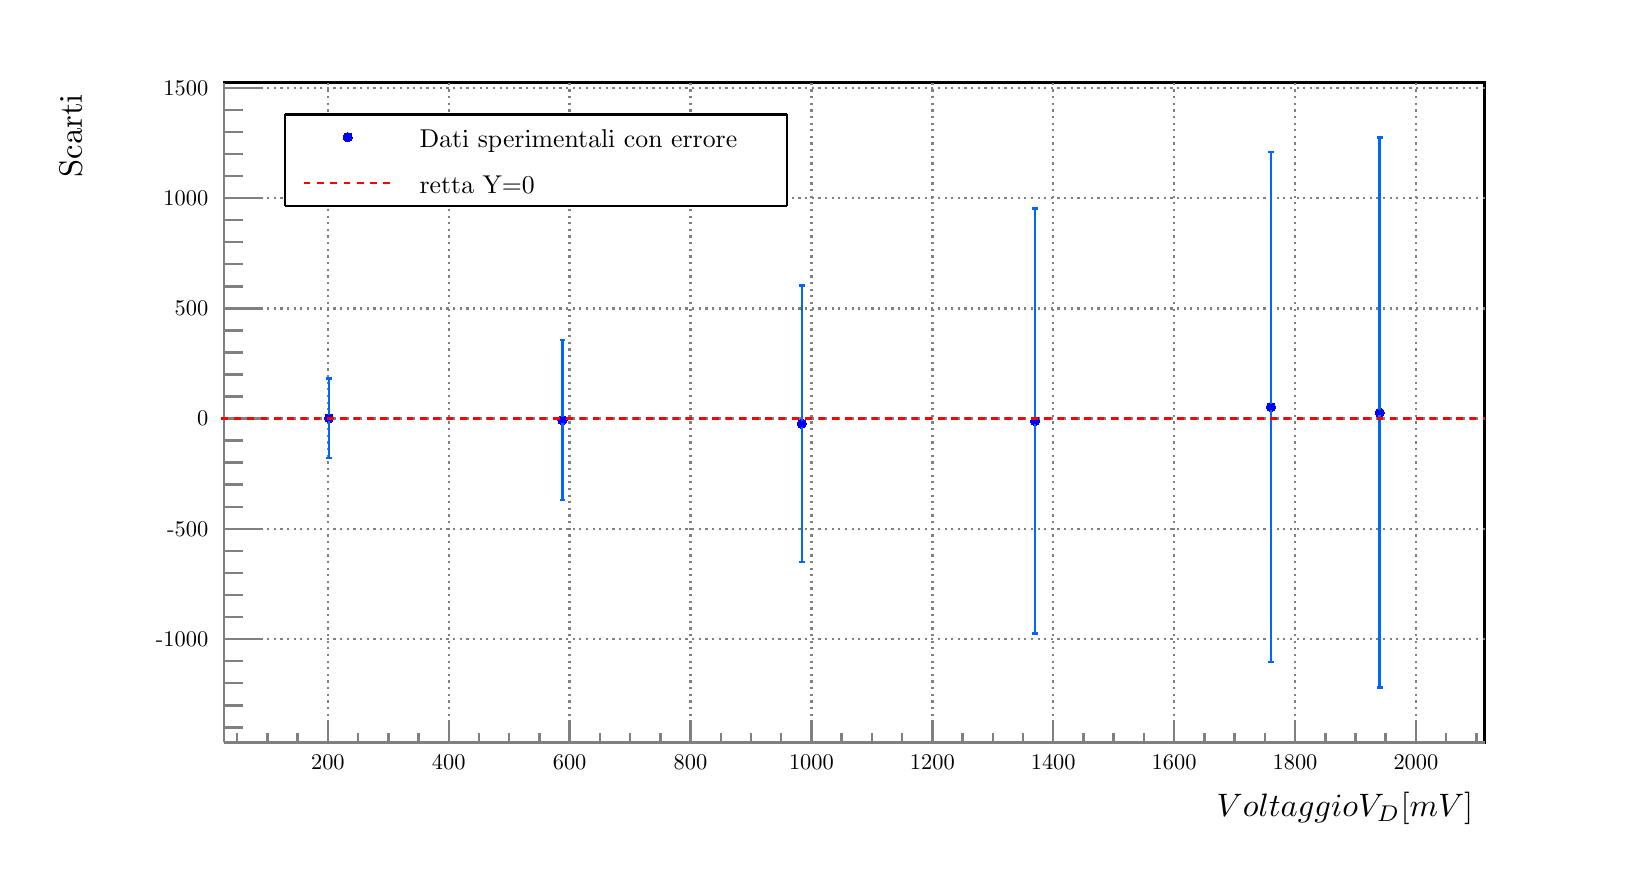
\begin{tikzpicture}
\pgfdeclareplotmark{cross} {
\pgfpathmoveto{\pgfpoint{-0.3\pgfplotmarksize}{\pgfplotmarksize}}
\pgfpathlineto{\pgfpoint{+0.3\pgfplotmarksize}{\pgfplotmarksize}}
\pgfpathlineto{\pgfpoint{+0.3\pgfplotmarksize}{0.3\pgfplotmarksize}}
\pgfpathlineto{\pgfpoint{+1\pgfplotmarksize}{0.3\pgfplotmarksize}}
\pgfpathlineto{\pgfpoint{+1\pgfplotmarksize}{-0.3\pgfplotmarksize}}
\pgfpathlineto{\pgfpoint{+0.3\pgfplotmarksize}{-0.3\pgfplotmarksize}}
\pgfpathlineto{\pgfpoint{+0.3\pgfplotmarksize}{-1.\pgfplotmarksize}}
\pgfpathlineto{\pgfpoint{-0.3\pgfplotmarksize}{-1.\pgfplotmarksize}}
\pgfpathlineto{\pgfpoint{-0.3\pgfplotmarksize}{-0.3\pgfplotmarksize}}
\pgfpathlineto{\pgfpoint{-1.\pgfplotmarksize}{-0.3\pgfplotmarksize}}
\pgfpathlineto{\pgfpoint{-1.\pgfplotmarksize}{0.3\pgfplotmarksize}}
\pgfpathlineto{\pgfpoint{-0.3\pgfplotmarksize}{0.3\pgfplotmarksize}}
\pgfpathclose
\pgfusepathqstroke
}
\pgfdeclareplotmark{cross*} {
\pgfpathmoveto{\pgfpoint{-0.3\pgfplotmarksize}{\pgfplotmarksize}}
\pgfpathlineto{\pgfpoint{+0.3\pgfplotmarksize}{\pgfplotmarksize}}
\pgfpathlineto{\pgfpoint{+0.3\pgfplotmarksize}{0.3\pgfplotmarksize}}
\pgfpathlineto{\pgfpoint{+1\pgfplotmarksize}{0.3\pgfplotmarksize}}
\pgfpathlineto{\pgfpoint{+1\pgfplotmarksize}{-0.3\pgfplotmarksize}}
\pgfpathlineto{\pgfpoint{+0.3\pgfplotmarksize}{-0.3\pgfplotmarksize}}
\pgfpathlineto{\pgfpoint{+0.3\pgfplotmarksize}{-1.\pgfplotmarksize}}
\pgfpathlineto{\pgfpoint{-0.3\pgfplotmarksize}{-1.\pgfplotmarksize}}
\pgfpathlineto{\pgfpoint{-0.3\pgfplotmarksize}{-0.3\pgfplotmarksize}}
\pgfpathlineto{\pgfpoint{-1.\pgfplotmarksize}{-0.3\pgfplotmarksize}}
\pgfpathlineto{\pgfpoint{-1.\pgfplotmarksize}{0.3\pgfplotmarksize}}
\pgfpathlineto{\pgfpoint{-0.3\pgfplotmarksize}{0.3\pgfplotmarksize}}
\pgfpathclose
\pgfusepathqfillstroke
}
\pgfdeclareplotmark{newstar} {
\pgfpathmoveto{\pgfqpoint{0pt}{\pgfplotmarksize}}
\pgfpathlineto{\pgfqpointpolar{44}{0.5\pgfplotmarksize}}
\pgfpathlineto{\pgfqpointpolar{18}{\pgfplotmarksize}}
\pgfpathlineto{\pgfqpointpolar{-20}{0.5\pgfplotmarksize}}
\pgfpathlineto{\pgfqpointpolar{-54}{\pgfplotmarksize}}
\pgfpathlineto{\pgfqpointpolar{-90}{0.5\pgfplotmarksize}}
\pgfpathlineto{\pgfqpointpolar{234}{\pgfplotmarksize}}
\pgfpathlineto{\pgfqpointpolar{198}{0.5\pgfplotmarksize}}
\pgfpathlineto{\pgfqpointpolar{162}{\pgfplotmarksize}}
\pgfpathlineto{\pgfqpointpolar{134}{0.5\pgfplotmarksize}}
\pgfpathclose
\pgfusepathqstroke
}
\pgfdeclareplotmark{newstar*} {
\pgfpathmoveto{\pgfqpoint{0pt}{\pgfplotmarksize}}
\pgfpathlineto{\pgfqpointpolar{44}{0.5\pgfplotmarksize}}
\pgfpathlineto{\pgfqpointpolar{18}{\pgfplotmarksize}}
\pgfpathlineto{\pgfqpointpolar{-20}{0.5\pgfplotmarksize}}
\pgfpathlineto{\pgfqpointpolar{-54}{\pgfplotmarksize}}
\pgfpathlineto{\pgfqpointpolar{-90}{0.5\pgfplotmarksize}}
\pgfpathlineto{\pgfqpointpolar{234}{\pgfplotmarksize}}
\pgfpathlineto{\pgfqpointpolar{198}{0.5\pgfplotmarksize}}
\pgfpathlineto{\pgfqpointpolar{162}{\pgfplotmarksize}}
\pgfpathlineto{\pgfqpointpolar{134}{0.5\pgfplotmarksize}}
\pgfpathclose
\pgfusepathqfillstroke
}
\definecolor{c}{rgb}{1,1,1};
\draw [color=c, fill=c] (0,0) rectangle (20,10.4736);
\draw [color=c, fill=c] (2.48634,1.40255) rectangle (18.4973,9.78142);
\definecolor{c}{rgb}{0,0,0};
\draw [c,line width=0.9] (2.48634,1.40255) -- (2.48634,9.78142) -- (18.4973,9.78142) -- (18.4973,1.40255) -- (2.48634,1.40255);
\definecolor{c}{rgb}{1,1,1};
\draw [color=c, fill=c] (2.48634,1.40255) rectangle (18.4973,9.78142);
\definecolor{c}{rgb}{0,0,0};
\draw [c,line width=0.9] (2.48634,1.40255) -- (2.48634,9.78142) -- (18.4973,9.78142) -- (18.4973,1.40255) -- (2.48634,1.40255);
\definecolor{c}{rgb}{0.5,0.5,0.5};
\draw [c,line width=0.9] (2.48634,1.40255) -- (18.4973,1.40255);
\draw [c,dash pattern=on 0.80pt off 1.60pt ,line width=0.9] (3.80523,9.78142) -- (3.80523,1.40255);
\draw [c,dash pattern=on 0.80pt off 1.60pt ,line width=0.9] (5.34061,9.78142) -- (5.34061,1.40255);
\draw [c,dash pattern=on 0.80pt off 1.60pt ,line width=0.9] (6.87599,9.78142) -- (6.87599,1.40255);
\draw [c,dash pattern=on 0.80pt off 1.60pt ,line width=0.9] (8.41137,9.78142) -- (8.41137,1.40255);
\draw [c,dash pattern=on 0.80pt off 1.60pt ,line width=0.9] (9.94674,9.78142) -- (9.94674,1.40255);
\draw [c,dash pattern=on 0.80pt off 1.60pt ,line width=0.9] (11.4821,9.78142) -- (11.4821,1.40255);
\draw [c,dash pattern=on 0.80pt off 1.60pt ,line width=0.9] (13.0175,9.78142) -- (13.0175,1.40255);
\draw [c,dash pattern=on 0.80pt off 1.60pt ,line width=0.9] (14.5529,9.78142) -- (14.5529,1.40255);
\draw [c,dash pattern=on 0.80pt off 1.60pt ,line width=0.9] (16.0883,9.78142) -- (16.0883,1.40255);
\draw [c,dash pattern=on 0.80pt off 1.60pt ,line width=0.9] (17.6236,9.78142) -- (17.6236,1.40255);
\draw [c,dash pattern=on 0.80pt off 1.60pt ,line width=0.9] (3.80523,9.78142) -- (3.80523,1.40255);
\draw [c,dash pattern=on 0.80pt off 1.60pt ,line width=0.9] (17.6236,9.78142) -- (17.6236,1.40255);
\draw [c,line width=0.9] (2.48634,1.40255) -- (2.48634,9.78142);
\draw [c,dash pattern=on 0.80pt off 1.60pt ,line width=0.9] (18.4973,2.71523) -- (2.48634,2.71523);
\draw [c,dash pattern=on 0.80pt off 1.60pt ,line width=0.9] (18.4973,4.11561) -- (2.48634,4.11561);
\draw [c,dash pattern=on 0.80pt off 1.60pt ,line width=0.9] (18.4973,5.516) -- (2.48634,5.516);
\draw [c,dash pattern=on 0.80pt off 1.60pt ,line width=0.9] (18.4973,6.91639) -- (2.48634,6.91639);
\draw [c,dash pattern=on 0.80pt off 1.60pt ,line width=0.9] (18.4973,8.31677) -- (2.48634,8.31677);
\draw [c,dash pattern=on 0.80pt off 1.60pt ,line width=0.9] (18.4973,9.71716) -- (2.48634,9.71716);
\draw [c,dash pattern=on 0.80pt off 1.60pt ,line width=0.9] (18.4973,2.71523) -- (2.48634,2.71523);
\draw [c,dash pattern=on 0.80pt off 1.60pt ,line width=0.9] (18.4973,9.71716) -- (2.48634,9.71716);
\draw [c,line width=0.9] (2.48634,1.40255) -- (18.4973,1.40255);
\draw [c,line width=0.9] (3.80523,1.65409) -- (3.80523,1.40255);
\draw [c,line width=0.9] (4.18907,1.52832) -- (4.18907,1.40255);
\draw [c,line width=0.9] (4.57292,1.52832) -- (4.57292,1.40255);
\draw [c,line width=0.9] (4.95676,1.52832) -- (4.95676,1.40255);
\draw [c,line width=0.9] (5.34061,1.65409) -- (5.34061,1.40255);
\draw [c,line width=0.9] (5.72445,1.52832) -- (5.72445,1.40255);
\draw [c,line width=0.9] (6.1083,1.52832) -- (6.1083,1.40255);
\draw [c,line width=0.9] (6.49214,1.52832) -- (6.49214,1.40255);
\draw [c,line width=0.9] (6.87599,1.65409) -- (6.87599,1.40255);
\draw [c,line width=0.9] (7.25983,1.52832) -- (7.25983,1.40255);
\draw [c,line width=0.9] (7.64368,1.52832) -- (7.64368,1.40255);
\draw [c,line width=0.9] (8.02752,1.52832) -- (8.02752,1.40255);
\draw [c,line width=0.9] (8.41137,1.65409) -- (8.41137,1.40255);
\draw [c,line width=0.9] (8.79521,1.52832) -- (8.79521,1.40255);
\draw [c,line width=0.9] (9.17905,1.52832) -- (9.17905,1.40255);
\draw [c,line width=0.9] (9.5629,1.52832) -- (9.5629,1.40255);
\draw [c,line width=0.9] (9.94674,1.65409) -- (9.94674,1.40255);
\draw [c,line width=0.9] (10.3306,1.52832) -- (10.3306,1.40255);
\draw [c,line width=0.9] (10.7144,1.52832) -- (10.7144,1.40255);
\draw [c,line width=0.9] (11.0983,1.52832) -- (11.0983,1.40255);
\draw [c,line width=0.9] (11.4821,1.65409) -- (11.4821,1.40255);
\draw [c,line width=0.9] (11.866,1.52832) -- (11.866,1.40255);
\draw [c,line width=0.9] (12.2498,1.52832) -- (12.2498,1.40255);
\draw [c,line width=0.9] (12.6337,1.52832) -- (12.6337,1.40255);
\draw [c,line width=0.9] (13.0175,1.65409) -- (13.0175,1.40255);
\draw [c,line width=0.9] (13.4013,1.52832) -- (13.4013,1.40255);
\draw [c,line width=0.9] (13.7852,1.52832) -- (13.7852,1.40255);
\draw [c,line width=0.9] (14.169,1.52832) -- (14.169,1.40255);
\draw [c,line width=0.9] (14.5529,1.65409) -- (14.5529,1.40255);
\draw [c,line width=0.9] (14.9367,1.52832) -- (14.9367,1.40255);
\draw [c,line width=0.9] (15.3206,1.52832) -- (15.3206,1.40255);
\draw [c,line width=0.9] (15.7044,1.52832) -- (15.7044,1.40255);
\draw [c,line width=0.9] (16.0883,1.65409) -- (16.0883,1.40255);
\draw [c,line width=0.9] (16.4721,1.52832) -- (16.4721,1.40255);
\draw [c,line width=0.9] (16.8559,1.52832) -- (16.8559,1.40255);
\draw [c,line width=0.9] (17.2398,1.52832) -- (17.2398,1.40255);
\draw [c,line width=0.9] (17.6236,1.65409) -- (17.6236,1.40255);
\draw [c,line width=0.9] (3.80523,1.65409) -- (3.80523,1.40255);
\draw [c,line width=0.9] (3.42138,1.52832) -- (3.42138,1.40255);
\draw [c,line width=0.9] (3.03754,1.52832) -- (3.03754,1.40255);
\draw [c,line width=0.9] (2.6537,1.52832) -- (2.6537,1.40255);
\draw [c,line width=0.9] (17.6236,1.65409) -- (17.6236,1.40255);
\draw [c,line width=0.9] (18.0075,1.52832) -- (18.0075,1.40255);
\draw [c,line width=0.9] (18.3913,1.52832) -- (18.3913,1.40255);
\definecolor{c}{rgb}{0,0,0};
\draw [anchor=base] (3.80523,1.05692) node[scale=0.809097, color=c, rotate=0]{200};
\draw [anchor=base] (5.34061,1.05692) node[scale=0.809097, color=c, rotate=0]{400};
\draw [anchor=base] (6.87599,1.05692) node[scale=0.809097, color=c, rotate=0]{600};
\draw [anchor=base] (8.41137,1.05692) node[scale=0.809097, color=c, rotate=0]{800};
\draw [anchor=base] (9.94674,1.05692) node[scale=0.809097, color=c, rotate=0]{1000};
\draw [anchor=base] (11.4821,1.05692) node[scale=0.809097, color=c, rotate=0]{1200};
\draw [anchor=base] (13.0175,1.05692) node[scale=0.809097, color=c, rotate=0]{1400};
\draw [anchor=base] (14.5529,1.05692) node[scale=0.809097, color=c, rotate=0]{1600};
\draw [anchor=base] (16.0883,1.05692) node[scale=0.809097, color=c, rotate=0]{1800};
\draw [anchor=base] (17.6236,1.05692) node[scale=0.809097, color=c, rotate=0]{2000};
\draw [anchor= east] (18.4973,0.564663) node[scale=1.17319, color=c, rotate=0]{$Voltaggio V_{D} [mV]$};
\definecolor{c}{rgb}{0.5,0.5,0.5};
\draw [c,line width=0.9] (2.48634,1.40255) -- (2.48634,9.78142);
\draw [c,line width=0.9] (2.96634,2.71523) -- (2.48634,2.71523);
\draw [c,line width=0.9] (2.72634,2.99531) -- (2.48634,2.99531);
\draw [c,line width=0.9] (2.72634,3.27538) -- (2.48634,3.27538);
\draw [c,line width=0.9] (2.72634,3.55546) -- (2.48634,3.55546);
\draw [c,line width=0.9] (2.72634,3.83554) -- (2.48634,3.83554);
\draw [c,line width=0.9] (2.96634,4.11561) -- (2.48634,4.11561);
\draw [c,line width=0.9] (2.72634,4.39569) -- (2.48634,4.39569);
\draw [c,line width=0.9] (2.72634,4.67577) -- (2.48634,4.67577);
\draw [c,line width=0.9] (2.72634,4.95585) -- (2.48634,4.95585);
\draw [c,line width=0.9] (2.72634,5.23592) -- (2.48634,5.23592);
\draw [c,line width=0.9] (2.96634,5.516) -- (2.48634,5.516);
\draw [c,line width=0.9] (2.72634,5.79608) -- (2.48634,5.79608);
\draw [c,line width=0.9] (2.72634,6.07616) -- (2.48634,6.07616);
\draw [c,line width=0.9] (2.72634,6.35623) -- (2.48634,6.35623);
\draw [c,line width=0.9] (2.72634,6.63631) -- (2.48634,6.63631);
\draw [c,line width=0.9] (2.96634,6.91639) -- (2.48634,6.91639);
\draw [c,line width=0.9] (2.72634,7.19647) -- (2.48634,7.19647);
\draw [c,line width=0.9] (2.72634,7.47654) -- (2.48634,7.47654);
\draw [c,line width=0.9] (2.72634,7.75662) -- (2.48634,7.75662);
\draw [c,line width=0.9] (2.72634,8.0367) -- (2.48634,8.0367);
\draw [c,line width=0.9] (2.96634,8.31677) -- (2.48634,8.31677);
\draw [c,line width=0.9] (2.72634,8.59685) -- (2.48634,8.59685);
\draw [c,line width=0.9] (2.72634,8.87693) -- (2.48634,8.87693);
\draw [c,line width=0.9] (2.72634,9.15701) -- (2.48634,9.15701);
\draw [c,line width=0.9] (2.72634,9.43708) -- (2.48634,9.43708);
\draw [c,line width=0.9] (2.96634,9.71716) -- (2.48634,9.71716);
\draw [c,line width=0.9] (2.96634,2.71523) -- (2.48634,2.71523);
\draw [c,line width=0.9] (2.72634,2.43515) -- (2.48634,2.43515);
\draw [c,line width=0.9] (2.72634,2.15507) -- (2.48634,2.15507);
\draw [c,line width=0.9] (2.72634,1.875) -- (2.48634,1.875);
\draw [c,line width=0.9] (2.72634,1.59492) -- (2.48634,1.59492);
\draw [c,line width=0.9] (2.96634,9.71716) -- (2.48634,9.71716);
\definecolor{c}{rgb}{0,0,0};
\draw [anchor= east] (2.38634,2.71523) node[scale=0.809097, color=c, rotate=0]{-1000};
\draw [anchor= east] (2.38634,4.11561) node[scale=0.809097, color=c, rotate=0]{-500};
\draw [anchor= east] (2.38634,5.516) node[scale=0.809097, color=c, rotate=0]{0};
\draw [anchor= east] (2.38634,6.91639) node[scale=0.809097, color=c, rotate=0]{500};
\draw [anchor= east] (2.38634,8.31677) node[scale=0.809097, color=c, rotate=0]{1000};
\draw [anchor= east] (2.38634,9.71716) node[scale=0.809097, color=c, rotate=0]{1500};
\draw [anchor= east] (0.539162,9.78142) node[scale=1.17319, color=c, rotate=90]{Scarti};
\definecolor{c}{rgb}{0,0,1};
\foreach \P in {(3.82058,5.52119), (6.78386,5.4976), (9.82391,5.45133), (12.7872,5.48375), (15.7812,5.66394), (17.163,5.59199)}{\draw[mark options={color=c,fill=c},mark size=1.681682pt, line width=0.000000pt, mark=*] plot coordinates {\P};}
\definecolor{c}{rgb}{0,0.4,1};
\draw [c,line width=0.9] (3.82058,5.55762) -- (3.82058,6.02607);
\draw [c,line width=0.9] (3.78415,6.02607) -- (3.85701,6.02607);
\draw [c,line width=0.9] (3.82058,5.48477) -- (3.82058,5.01632);
\draw [c,line width=0.9] (3.78415,5.01632) -- (3.85701,5.01632);
\draw [c,line width=0.9] (6.78386,5.53403) -- (6.78386,6.51191);
\draw [c,line width=0.9] (6.74743,6.51191) -- (6.82029,6.51191);
\draw [c,line width=0.9] (6.78386,5.46117) -- (6.78386,4.48328);
\draw [c,line width=0.9] (6.74743,4.48328) -- (6.82029,4.48328);
\draw [c,line width=0.9] (9.82391,5.48776) -- (9.82391,7.20536);
\draw [c,line width=0.9] (9.78748,7.20536) -- (9.86034,7.20536);
\draw [c,line width=0.9] (9.82391,5.4149) -- (9.82391,3.6973);
\draw [c,line width=0.9] (9.78748,3.6973) -- (9.86034,3.6973);
\draw [c,line width=0.9] (12.7872,5.52018) -- (12.7872,8.18133);
\draw [c,line width=0.9] (12.7508,8.18133) -- (12.8236,8.18133);
\draw [c,line width=0.9] (12.7872,5.44732) -- (12.7872,2.78616);
\draw [c,line width=0.9] (12.7508,2.78616) -- (12.8236,2.78616);
\draw [c,line width=0.9] (15.7812,5.70037) -- (15.7812,8.90477);
\draw [c,line width=0.9] (15.7448,8.90477) -- (15.8176,8.90477);
\draw [c,line width=0.9] (15.7812,5.62751) -- (15.7812,2.4231);
\draw [c,line width=0.9] (15.7448,2.4231) -- (15.8176,2.4231);
\draw [c,line width=0.9] (17.163,5.62842) -- (17.163,9.08318);
\draw [c,line width=0.9] (17.1266,9.08318) -- (17.1995,9.08318);
\draw [c,line width=0.9] (17.163,5.55556) -- (17.163,2.10079);
\draw [c,line width=0.9] (17.1266,2.10079) -- (17.1995,2.10079);
\definecolor{c}{rgb}{1,0,0};
\draw [c,dash pattern=on 2.40pt off 2.40pt ,line width=0.9] (2.44642,5.516) -- (18.5065,5.516);
\definecolor{c}{rgb}{1,1,1};
\draw [color=c, fill=c] (3.26047,8.21494) rectangle (9.6357,9.38069);
\definecolor{c}{rgb}{0,0,0};
\draw [c,line width=0.9] (3.26047,8.21494) -- (9.6357,8.21494);
\draw [c,line width=0.9] (9.6357,8.21494) -- (9.6357,9.38069);
\draw [c,line width=0.9] (9.6357,9.38069) -- (3.26047,9.38069);
\draw [c,line width=0.9] (3.26047,9.38069) -- (3.26047,8.21494);
\draw [anchor=base west] (4.85428,8.95811) node[scale=0.930461, color=c, rotate=0]{Dati sperimentali con errore};
\definecolor{c}{rgb}{0,0,1};
\foreach \P in {(4.05738,9.08925)}{\draw[mark options={color=c,fill=c},mark size=1.681682pt, line width=0.000000pt, mark=*] plot coordinates {\P};}
\definecolor{c}{rgb}{0,0,0};
\draw [anchor=base west] (4.85428,8.37523) node[scale=0.930461, color=c, rotate=0]{retta Y=0};
\definecolor{c}{rgb}{1,0,0};
\draw [c,dash pattern=on 2.40pt off 2.40pt ,line width=0.9] (3.49954,8.50638) -- (4.61521,8.50638);
\end{tikzpicture}
